\documentclass{article}

\usepackage{arxiv}
\usepackage[utf8]{inputenc}
\usepackage[T1]{fontenc}
\usepackage{url}
\usepackage{booktabs}
\usepackage{amsfonts}
\usepackage{nicefrac}
\usepackage{microtype}
\usepackage{graphicx}
\usepackage[font=small,labelfont=bf]{caption}
\usepackage{cite}
\usepackage{pdflscape}
\usepackage{listings}
\usepackage{outlines}
\usepackage{tikz}
\usepackage{epigraph}
\usepackage{natbib} 
\usepackage{url}
\usepackage{algorithm,algpseudocode}

\newcommand*\circled[1]{\tikz[baseline=(char.base)]{
		\node[shape=circle,draw,inner sep=1pt] (char) {#1};}}

\title{Lineage of tiered data in Apache Kafka}

\begin{document}
\maketitle \thispagestyle{fancy2}
\begin{abstract}
	The objective of this document is to elaborate on the design of "tiered storage" to ensure the lineage of logs in Apache Kafka is preserved  when segments are moved to and accessed from external storage tiers.
\end{abstract}

\tableofcontents

\newpage
\section{Motivation}
\epigraph{\textit{"At its heart a Kafka partition is a replicated log"}}{Apache Kafka online documentation \cite{RD1}}

As stated in the reference documentation and echoed in \cite{KDG}, replication in Apache Kafka is one of its most fundamental characteristic. The replication protocol which Kafka implements and the guarantees it provides are well documented, and explains how and why a consistent lineage for a topic-partition is preserved across its replicas irrespective of the nature and frequency of fail-overs this topic-partition experiences \cite{KIP101}\cite{KIP279}.

Over time, Kafka gracefully evolved and built on top of existing replication protocol to strengthen replication semantic. Introducing a feature which would weaken the replication guarantees offered by Kafka would not be acceptable. One of the premise of the integration of data tiering in Apache Kafka is to provide users with a uniform experience of access to data irrespective of its provenance (the storage tier where it comes from). This requires the data lineage to be kept consistent when information is read from tiered segments in addition to local segments. The specifications which apply to local replicas are still honored when tiered segments contribute to a replica's lineage.

This document assumes some level of familiarity with the replication protocol implemented in Kafka and how replica lineage is maintained across replicas. At a very high level, this protocol is based on \textit{log truncation}, which relies on replica history, materialized by a list of generation to start offset vectors, which evolves with cluster events and leadership migration. At a given point in time, the lineage of the log of a topic-partition is that of the leader replica of that topic-partition. It is possible for the end offset of the log to decrease when leadership of a topic-partition is migrated. Truncation prevents divergences between replicas.

\section{Introducing example}

The following discussion is based on an example which consists in a topic-partition with three replicas and multiple leadership migrations. The lineage tree of the topic-partition is provided in diagrams along with the leadership assignments throughout the sequence of generations for this topic-partition.

\subsection{Notations and simplifications}

\textbf{Serialized offsets}

In this example, offsets are selected from the available replicas at points of interest. An offset is written "$\theta$" and informally indexed such that $\theta_{i+1}$ is written on a replica "after" $\theta_i$ for any given index $i$. The use of leader epochs makes this serialization possible and ensure the word \textit{after} is meaningful in this context. Note that $(\theta_i)_{i \in \mathbb{N}}$ is not necessarily monotonic. 

\textbf{Generations}

A leader epoch is written $g$ and is indexed such that $g_{i+1}$ is "younger" than $g_i$. Note that, for simplicity, the exact sequence of incremental leader epochs is not reproduced. For instance, when replica 2 and 3 go offline in figure \ref{fig:lineage-tree-1}, the leader epoch of the topic-partition is expected to be incremented at least twice, but we will simply refer to the new leader epoch as $g_2$ even if it differs from $g_1$ by more than one logical increment.

\subsection{Lineage tree}

\label{lineage_tree}
\textbf{Figure \ref{fig:lineage-tree-1}} provides the lineage tree of the log, where each replica exhibits a specific history.
The timeline of events which led to this tree are as follows:

\begin{outline}[enumerate]
\1 The root of the tree corresponds to the subsegment in the range $[\theta_1, \theta_2]$, which is assumed to be common to all three replicas.
\1 At generation $g_2$, replicas 2 and 3 become offline and replica 1 ingest records from $\theta_{2} + 1$ to beyond $\theta_3$. The segment with base offset $\theta_1$ and end offset $\theta_3$ is offloaded by replica 1\footnote{Here, the word \textit{replica} informally refers to the hosting \textit{broker}.}. The information required to know how that segment participated to the lineage of the replica needs to be preserved and leader epochs $g_1$ and $g_2$ along with start and end offsets are kept as part of the tiered segment metadata.
\1 Replica 1 becomes offline and replica 2 and 3 now contribute to the ISR set. Replica 3 is the leader. The segment with the offset range $[\theta_1, \theta_4]$ is offloaded and its generational metadata is recorded.
\1 Replica 2 falls behind and is moved out of ISR. Replica 3 continues to ingest and offload the segment ranging from offsets $[\theta_4 + 1, \theta_5]$ at generation $g_4$. This is possible because the ISR is reduced to its leader and the leader high watermark can freely moves forward.
\1 Leadership is transferred to replica 2 and replica 3 is put offline. The ISR set is now $\{2\}$. Data continues to be ingested.
\1 Replica 3 is back online. Generation is incremented to $g_6$ when it joins the cluster. Truncation is performed on the replica, which physically deletes the segment $[\theta_{5}+1, \theta_{5}+2]$. The segment the replica offloaded at generation $g_4$ is only in the external storage at truncation time. This segment is now "\textit{orphan}", because no matter the following life events affecting the cluster, there is no going back and that part of the lineage is forever discarded. Another way to see it is that the edge from the prefix $[\theta_2+1,\theta_4]$ to $[\theta_4+1,\theta_6]$ in the lineage tree can be removed.
\1 The segment $[\theta_2+1,\theta_6]$ is rolled over and eventually become eligible for tiering. It is offloaded by replica 2 and its generational metadata is recorded.
\end{outline}

The content of the tiered storage after these events is represented in \textbf{figure \ref{fig:tiered-storage}}, with the representation of the generational metadata associated to the tiered segments as a graph $\mathcal{G}=(\theta,g)$ which provides the ranges of offsets of the tiered segments along with the leader epochs at ingestion time.

\begin{figure}[H]
	\centering
	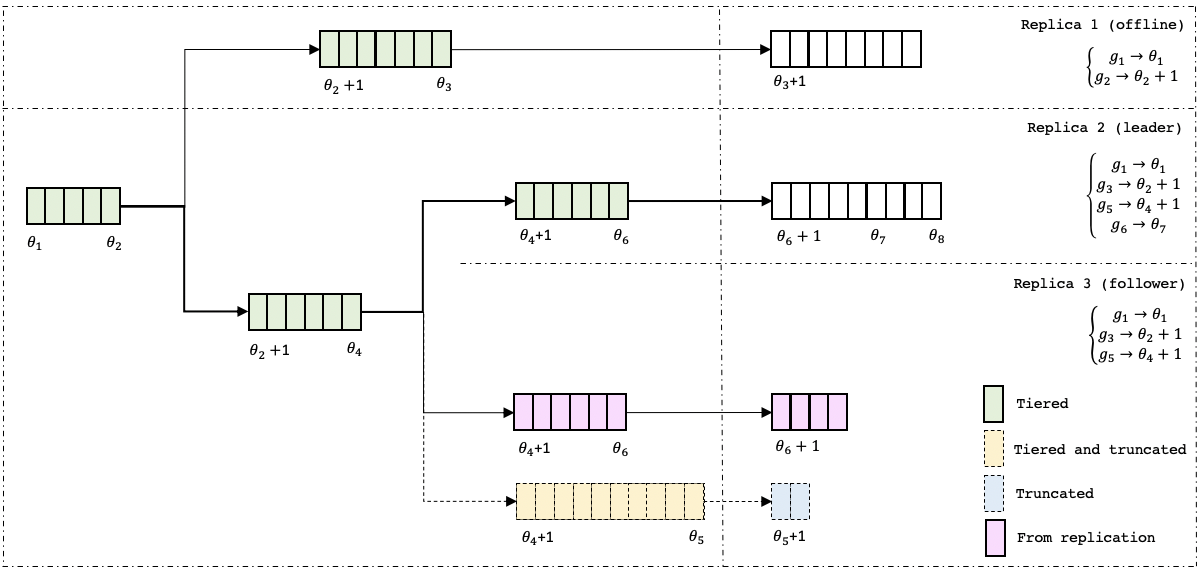
\includegraphics[scale=0.45]{lineage-tree-1.png}
	\captionof{figure}{Lineage tree of the topic-partition while replica 1 is offline. The generation-to-start-offset vectors, which build the leader epoch cache, are represented on the right.}
	\label{fig:lineage-tree-1}
\end{figure}

\begin{figure}[H]
	\centering
	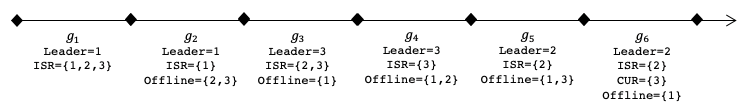
\includegraphics[scale=0.6]{seq-generations.png}
	\captionof{figure}{Lineage tree of the topic-partition while replica 1 is offline.}
	\label{fig:seq-generations}
\end{figure}

\begin{figure}[H]
	\centering
	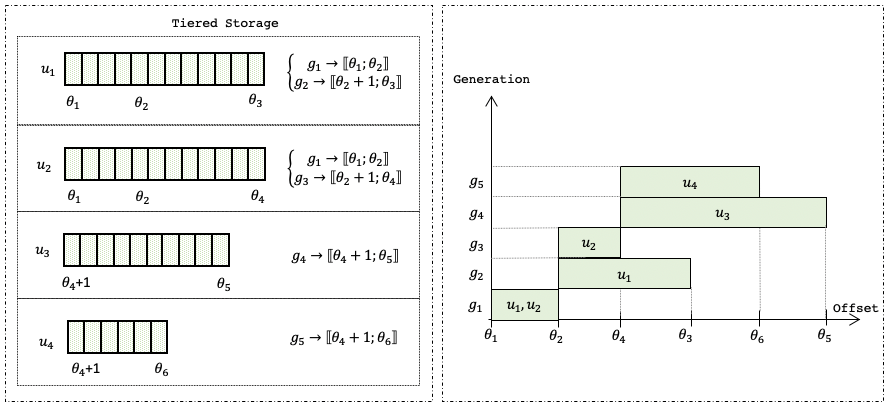
\includegraphics[scale=0.54]{tiered-storage.png}
	\captionof{figure}{On the left: tiered segments. On the right: a representation of lineage information associated to these segments.}
	\label{fig:tiered-storage}
\end{figure}

\newpage
\section{Lineage reconcilation with tiered segments}

\subsection{Reconcilation between local and tiered segments on \texttt{become-leader}}

\subsubsection{Remote End Offset}

A replica which becomes the leader of a topic-partition, and detects some segments for that topic-partition are tiered, needs to identify which parts of its lineage are present in the tiered storage. 

As such, the replica which becomes leader needs to find the latest epoch which is common to tiered segments and the local epoch cache, following an approach similar to the resolution of the truncation offset \cite{KIP279}. It then resolves an offset depending on the relative position of the latest offset of the tiered segments and the local end offset at generation $g$.

The potential use cases are enumerated figure \ref{fig:become-leader}. Note that the configurations \circled{B}, \circled{C}, \circled{D}, \circled{E}, \circled{F} and \circled{G} correspond to the interval trichotomy and altogether, guarantee the exhaustive coverage (\cite{CLR} p.349) of all possible strutural cases. Additionally, note that figure \ref{fig:become-leader} does \textit{not} represent segments but sections of the log which were produced at a given generation. In order to refer to the offsets of interest, the following notations are used:

\begin{itemize}
	\item $\hat{\theta}_S(g)$ is the first offset for the generation $g$ in the tiered storage.
	\item $\hat{\theta}_E(g)$ is the last offset for the generation $g$ in the tiered storage.
	\item $\theta_{l,S}(g)$ is the local start offset for the leader epoch $g$ (inclusive) on the leader replica.
	\item $\theta_{l,E}(g)$ is the local end offset for the leader epoch $g$ (inclusive) on the leader replica.
\end{itemize} 

\begin{figure}[h!]
	\centering
	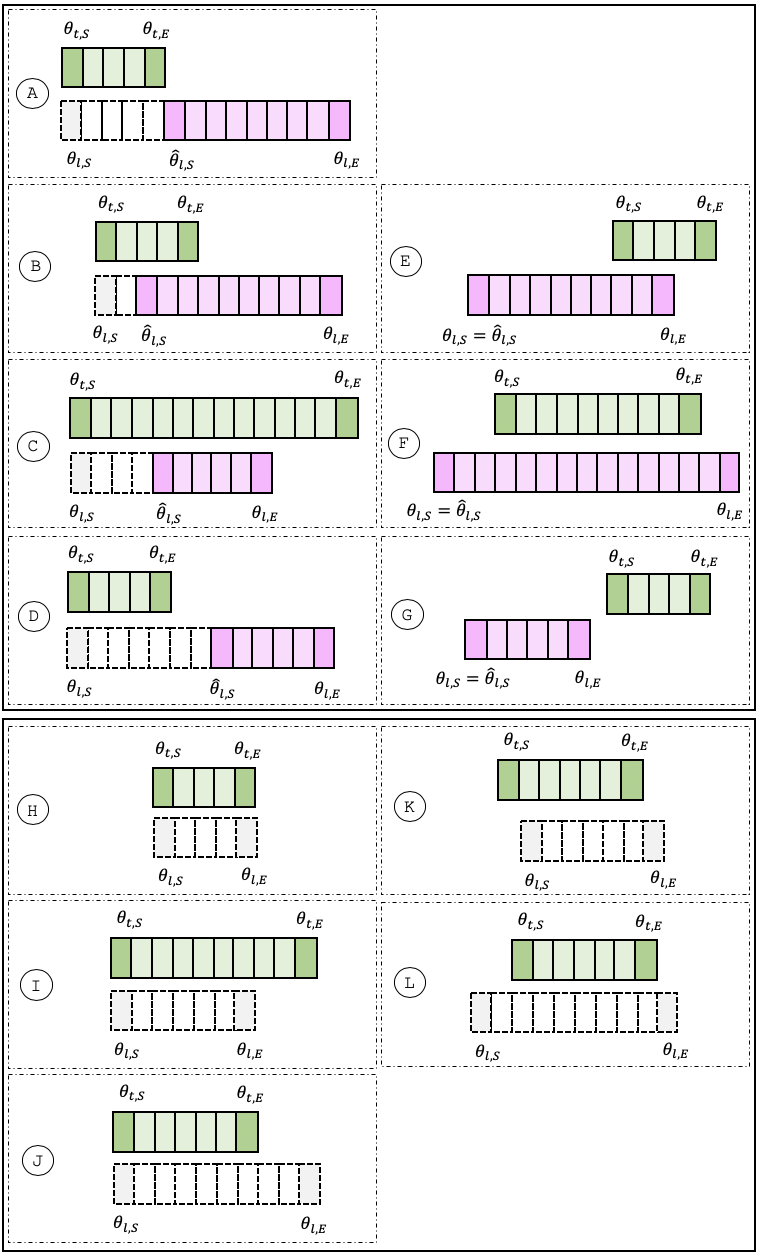
\includegraphics[scale=0.55]{become-leader.png}
	\captionof{figure}{.}
	\label{fig:become-leader}
\end{figure}

\begin{outline}[enumerate]
	\1 \textbf{Case \circled{A}}: $\hat{\theta}_E(g) = \theta_{l,S}(g) - 1$. This can be a usual case encountered when leadership of the topic-partition is migrated to a previously in-sync replica subject to the same local eviction sequence as the previous leader.
	\1 \textbf{Case \circled{B}}:  $\hat{\theta}_S(g) \leq \theta_{l,S}(g) < \hat{\theta}_E(g) \leq \theta_{l,E}(g)$. This can happen for instance if a tiered segment was not deleted on the new leader replica, or if the base offsets of the segments of the replica were not perfectly aligned with those of the previous leader, resulting in shifted roll-overs and deletion of local segments.
	\1 \textbf{Case \circled{C}}: $\hat{\theta}_S(g) \leq \theta_{l,S}(g) \leq \theta_{l,E}(g) < \hat{\theta}_E(g)$. This can happen if the new leader replica was previously out of the ISR set, but elected as a leader.
	\1 \textbf{Case \circled{D}}:  $\hat{\theta}_E(g) < \theta_{l,S}(g)$. A gap separates the local start offset from the latest offset at generation $g$. This could be the result of a misconfiguration which led to the premature eviction of local segments on the new leader replica.
	\1 \textbf{Case \circled{E}}, \textbf{Case \circled{F}} and \textbf{Case \circled{G}}: Pathological cases where the leader replica contains offsets preceding the earliest offset on the tiered storage at generation $g$. Segment tiering will ensure segments are sequentially delivered to the tiered storage, such that a segment is tiered only if the preceding segment has been successfully offloaded. However, these cases can still happen, for instance if segments were deleted from the tiered storage but kept locally on the leader replica.	
	\1 \textbf{Case \circled{E}}:  No common epoch can be found between tiered segments and the local epochs, no part of the local log is present in the tiered storage. That could be the case that historically, no part of the replica has ever been offloaded \circled{E.1}. However, there could be tiered segments which lineage was removed from the local epoch cache (log prefix truncation via \texttt{LeaderEpochFileCache\#truncateFromStart}) \circled{E.2}.
\end{outline}

In order to handle case \circled{E.2}, the epoch to start offset vectors for the epochs which are fully "tiered" (i.e. for which all segments are in the external storage and do not have remaining local copy) will be preserved. This will be in a file different from the local epoch cache to ensure no conflict can be introduced with existing functionalities.

The new leader will then derive the \textit{remote end offset} (\textbf{REO}), which is relative to a given leader epoch.

\begin{outline}[enumerate]
	\1 \textbf{Case \circled{A}}: The REO can be set to $\theta_R + 1$ (the same convention as for the LEO is adopted).
	\1 \textbf{Case \circled{B}}: The records present simultaneously in the external and local storage are guaranteed to match. The remote end offset will be set to $\theta_R + 1$. Any segment with base offset and end offset within the range $[\theta_S; \theta_R]$ will not be offloaded.
	\1 \textbf{Case \circled{C}}: In this case, we will want to consider the lineage of the new leader to be consistent with the existing behaviour with local segments. The REO will be set to $\theta_E + 1$, and the portion of the log in the range $[\theta_E + 1, \theta_R]$ will not be part of the current lineage (but is not deleted, because it can be reinstated as a part of the log by another leader in the future).
	\1 \textbf{Case \circled{D}}: The REO will be set to $\theta_R + 1$. No assumption should be made in other part of the system that the log concatenated from tiered and local segments is contiguous.
	\1 \textbf{Case \circled{E}}: The REO will be set to $-1$.
\end{outline}

\subsubsection{REO resolution}

An algorithm to resolve the REO (algorithm \ref{alg:reo}) which derived from the previous discussion is provided here. The following conventions are used:

\begin{itemize}
	\item $\phi$ is a map such that $\phi(g)$ represents the start offset of generation $g$ in the leader epoch cache.
	\item $\psi$ is a map such that $\psi(g)$ represents the end offset of all segments tiered for the generation $g$.
	\item The input of the algorithm are the list of generation to end offset $(g_k, \psi(g_k))_{k \in \{1,...,n\}}$, and the leader epoch cache $(h_l, \phi(h_l))_{l \in \{1,...,m\}}$.
	\item The function \textsc{EndOffsetFor} corresponds to \texttt{LeaderEpochFileCache\#endOffsetFor} and has implicitly access to the map $\phi$.
\end{itemize} 

\begin{algorithm}[h!]
	\caption{Resolution of the replica's REO on \texttt{become-leader}}
	\label{alg:reo}
	
	\begin{algorithmic}[1]
		\Function{FindRemoteEndOffset}{$(g_k)_{k \in \{1,..,n\}}$, $\psi$, $(h_h)_{h \in \{1,..,m\}}$, $\phi$}
			\State	$(i,j) \leftarrow (n-1,m-1)$
			\State	$(g_{-1}, h_{-1}) \leftarrow (-1,-1)$
			\\
			\While{$g_i \neq h_j$}
				\While{$g_i > h_j$}
					\State $i \leftarrow i - 1$
				\EndWhile
				\While{$h_j > g_i$}
					\State $j \leftarrow j - 1$
				\EndWhile
			\EndWhile
			\\
			\State // If there is no common lineage, return -1. Note that -1 is already used for sentinel leader epoch in multiple places.
			\State // Need to check conflicting semantic is avoided.
			\If{$i = -1$}
				\State \Return $-1$
			\EndIf
			\\
			\State // Get the latest offset of tiered segments and the local start offset, for the generation $g_i = h_j$.
			\State $\theta_R \leftarrow \psi(g_i)$
			\State $\theta_E \leftarrow  \textsc{EndOffsetFor}(h_j)$
			\\
			\If{$\theta_R > \theta_E$}
			\State \Return $\theta_E$ // Case \circled{C}
			\Else
			\State \Return $\theta_R + 1$ // Case \circled{A}, \circled{B}, \circled{D}
			\EndIf
			\\
		\EndFunction
	\end{algorithmic}	
\end{algorithm}

\newpage
\subsection{Reconciliation between local and tiered segments on \texttt{become-follower}}

\subsubsection{REO propagation}

When a replica initiates replication from a leader, it needs to know which part of the leader's lineage is tiered, to avoid replicating the corresponding segments from the leader.

Through the truncation protocol, the follower and leader collaboratively resolves the truncation offset $\theta_T(g)$ for the most recent generation $g$ they have in common. With local segments, the follower then starts fetching from the offset $\theta_T(g)$. Assume a segment which includes the truncation offset is tiered. The leader may contain a local copy of a segment which includes this offset, or it may only be available in the tiered storage. Irrespective of local availability, we expect the follower not to replicate it.

In order to adjust its initial fetch offset, the follower needs to know what the REO on the leader is. Additionally, the lineage characterization of the leader replica between the truncation offset and the REO needs to be copied and recorded by the follower. This is to preserve the current behaviour; for instance, to ensure the truncation protocol is not violated if the follower becomes a leader in the future, and its lineage between the truncation offset and the REO needs to be inspected to satisfy \texttt{OffsetsForLeaderEpoch} requests. Note that the lineage of the follower replica before the truncation offset is guaranteed to be identical to that of the leader.

There are similarities between the information required in our case and that of the truncation algorithm. The design alternative\footnote{https://tinyurl.com/yatnunsh} \circled{2} from KIP-279 \cite{KIP279} discusses how sub-sequences of the leader epoch to offset vector lists could be exchanged between a leader and follower in order to resolve the truncation offset. Our requirement is slightly different, since we only need the part of the lineage $\mathcal{L}$ between two defined offsets: $\theta_{T}$ and $\theta_{REO}$.

The characterizations of $\mathcal{L}$ are stored in the leader epoch cache, which is maintained locally by each replica. We chose not to create and maintain a copy of the leader epoch cache in an alternative destination, as this would require to implement the required coordination in the system to ensure both copy are kept in sync. Therefore, in order to access $\mathcal{L}$, the follower needs to retrieve it from the leader.

We propose the following approach. When the follower makes a \texttt{FetchRequest} starting with the truncation offset $\theta_T$, and the leader detects that $\theta_T < \theta_{REO}$, the \texttt{FetchResponse} returns a specific error which contains $\theta_{REO}$ and the part of the epoch cache between $\theta_T$ and $\theta_{REO}$. More formally, if the leader epoch cache is  $\mathcal{L}=\mathcal{G}\times\Theta=(g_i, \theta_S(g_i))_{i \in \{1,...,n\}}$, the response would contain the sublist $\mathcal{L'}=(g_i, \theta_S(g_i))_{i \in \{k,...,l\}} \sqsubset \mathcal{L}$ s.t. $\left\{
\begin{array}{l}
g_k=\max \texttt{} \{g \in \mathcal{G} \texttt{ } | \texttt{ } \theta_S(g) \leq \theta_{REO}\}\\
g_l=\min \texttt{} \{g \in \mathcal{G} \texttt{ } | \texttt{ } \theta_S(g) \geq \theta_T\}\\
\end{array}
\right.$

Consider the example described in section \ref{lineage_tree}. Assume the replica becomes online and starts replicating from replica 2.

\begin{figure}[H]
	\centering
	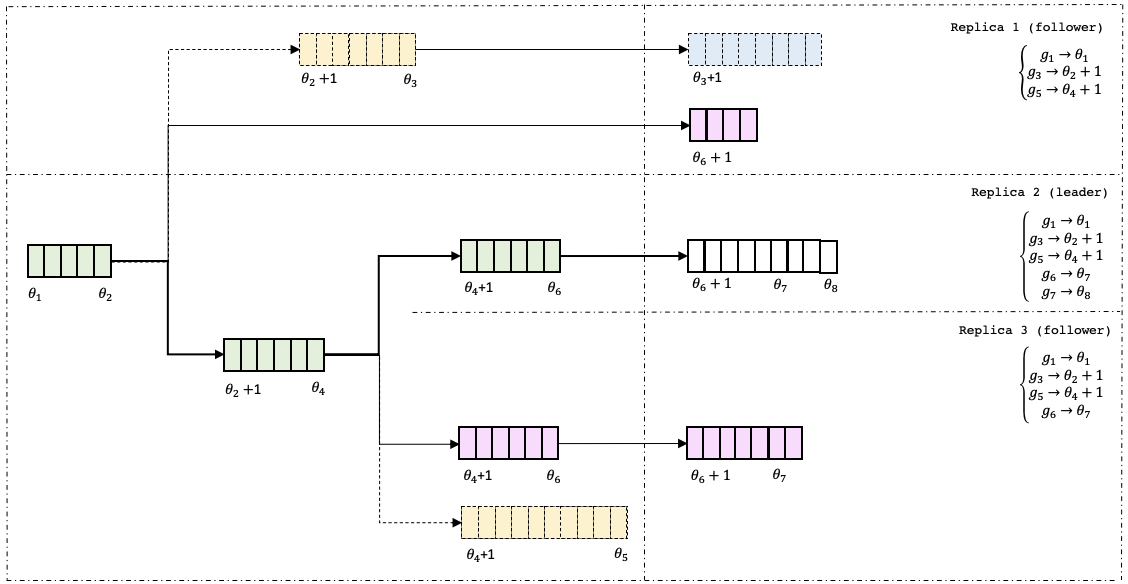
\includegraphics[scale=0.45]{lineage-tree-2.png}
	\captionof{figure}{}
	\label{fig:lineage-tree-2}
\end{figure}

Two RPCs from the follower are required to reconcile the current log lineage.

\begin{figure}[H]
	\centering
	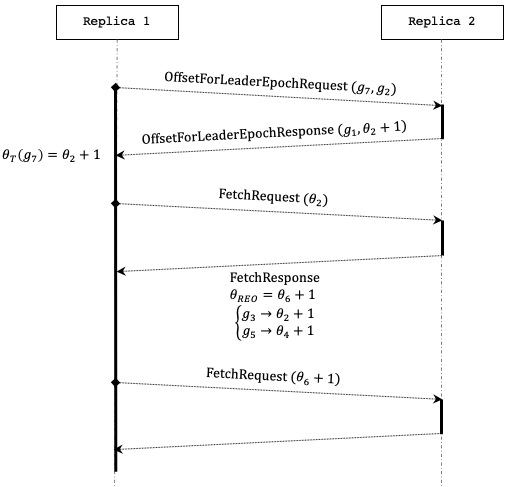
\includegraphics[scale=0.5]{RPCs.png}
	\captionof{figure}{}
	\label{fig:rpc}
\end{figure}


\newpage
\section{Coordination for Data Tiering}

\newpage
\section{Garbage collection of orphan segments}

\newpage
\bibliographystyle{plain}
\bibliography{tiered-storage-replication}{}
\end{document}
